\documentclass{article}
\usepackage{amsmath}
\usepackage{amssymb}
\usepackage{graphicx}
\usepackage{listings}
\usepackage{xcolor}
\usepackage{hyperref}

\title{Analytic Generative Design of Quasi-Symmetric Stellarators: An Inverse Riemannian Embedding Approach}
\author{David}
\date{\today}

\lstset{
    language=Python,
    basicstyle=\ttfamily\small,
    keywordstyle=\color{blue},
    stringstyle=\color{red},
    commentstyle=\color{green!50!black},
    showstringspaces=false,
    breaklines=true,
    frame=single,
    numbers=left
}

\begin{document}

\maketitle

\begin{abstract}
The commercial realization of stellarator fusion energy is hindered in part by the computational cost and non-convexity of 3D equilibrium and configuration optimization workflows. Many modern pipelines perform repeated high-dimensional searches (e.g., VMEC/STELLOPT-based loops) that are expensive and sensitive to initialization. This paper presents a deterministic, analytic framework for constructing \emph{near-axis} stellarator \emph{core geometries} that satisfy \textbf{quasi-symmetry (QS)} constraints \emph{to first order in a near-axis expansion (NAE)}. Using the NAE to invert the equilibrium/shaping relationships near the magnetic axis, we obtain a \textbf{Riccati ordinary differential equation} for a complex cross-section parameter $\sigma$ that determines the leading-order rotating-ellipse flux-surface geometry from magnetic-axis properties. The resulting generator reduces the initial core-shaping step from a high-dimensional variational search to integration of a single ODE together with a periodicity condition, enabling rapid generation of QA-consistent near-axis candidates that can seed subsequent full-equilibrium and coil-design stages. We provide a derivation summary and a Python implementation that constructs a Quasi-Axisymmetric (QA) near-axis configuration.
\end{abstract}

\section{Introduction}

The stellarator offers a pathway to steady-state nuclear fusion, free from the current-driven disruptions of the tokamak. However, a generic three-dimensional toroidal magnetic field lacks the continuous symmetry that yields simple single-particle invariants. A practical remedy is \textbf{quasi-symmetry (QS)}: a "hidden" symmetry in which the magnetic-field strength $B = |\mathbf{B}|$ depends on a single helicity angle in magnetic coordinates, despite the fully 3D geometry.

Traditional design follows an \textbf{Extrinsic} logic:
\[ \text{Guess Shape} \rightarrow \text{Solve Equilibrium} \rightarrow \text{Check Symmetry} \rightarrow \text{Iterate} \]
This process can consume substantial compute, especially when exploring configuration families. We propose an \textbf{intrinsic} logic:
\[ \text{Define Symmetry (Lie Group)} \rightarrow \text{Derive Metric} \rightarrow \text{Analytic Embedding} \rightarrow \text{Constructed Shape} \]

\subsection{Scope and contributions}

This work focuses on \emph{near-axis plasma geometry construction} (a first-order core shape consistent with QA/QS constraints), not a full 3D free-boundary equilibrium or magnetic-coil inverse design.
The intended use is as a fast \emph{generator} for candidate cores that can initialize or constrain subsequent equilibrium and coil stages.

Concretely, we contribute:
\begin{itemize}
    \item A concise presentation of the first-order QA near-axis generator in terms of a complex Riccati ODE for $\sigma$.
    \item A numerically robust implementation that computes axis curvature/torsion from analytic derivatives and integrates the generator with a periodicity-enforcement loop.
    \item A reproducible script that outputs a 3D surface visualization for rapid axis-family exploration.
\end{itemize}

\section{Mathematical Framework}

\subsection{The Lie Symmetry Constraint}

We utilize \textbf{Boozer Coordinates} $(\psi, \theta, \zeta)$. The magnetic field is:
\[ \mathbf{B} = \nabla \psi \times \nabla \theta + \iota(\psi) \nabla \zeta \times \nabla \psi \]
Quasi-Symmetry requires that the field magnitude $B$ is invariant under the generator $\mathbf{u} = M \partial_\theta + N \partial_\zeta$.
For \textbf{Quasi-Axisymmetry (QA)} $(M=1, N=0)$, the condition is $\partial_\zeta B = 0$.

In the constructive near-axis setting, the QS constraint is enforced order-by-order in the expansion parameter (minor radius) and is therefore \emph{approximate by design}: the result is QA-consistent to the order retained.

\subsection{Near-Axis Expansion (NAE)}

Since the global embedding problem is non-linear, we expand the solution around the magnetic axis $\mathbf{r}_0$. Let $s$ denote arc length along the axis, with curvature $\kappa(s)$ and torsion $\tau(s)$.
We define the flux surface cross-section using the vector $\mathbf{r}$ expanded in the effective radius $r$:
\[ \mathbf{r}(s, \theta, r) = \mathbf{r}_0(s) + r \left[ X(s, \theta)\mathbf{n}(s) + Y(s, \theta)\mathbf{b}(s) \right] + O(r^2) \]
where $(\mathbf{t}, \mathbf{n}, \mathbf{b})$ is the Frenet-Serret frame.

To satisfy MHD force balance $\mathbf{J} \times \mathbf{B} = \nabla p$ and the QS constraint simultaneously at first order, the flux-surface cross-section is a \textbf{rotating ellipse}. We parameterize this shape using a complex variable $\sigma(s)$ whose magnitude controls elongation and whose phase controls the rotation angle of the ellipse. A convenient mapping is
\[
E \equiv \frac{a}{b} = \frac{1+|\sigma|}{1-|\sigma|},
\]
where $a/b$ is the ellipse aspect ratio (elongation).

\subsection{The Master Riccati Equation (The "Generator")}

The relationship between axis geometry $(\kappa, \tau)$ and first-order cross-section shaping $(\sigma)$ is set by the near-axis equilibrium constraints together with the QA symmetry requirement. Following the near-axis QS construction of Garren and Boozer \cite{garren1991} and later developments (e.g. \cite{landreman2019}), the QA first-order shaping variable $\sigma$ satisfies a \textbf{Riccati ordinary differential equation}.

\textbf{Choice of evolution variable.} The underlying theory is naturally expressed in Boozer angles, but the implementation integrates in the \emph{geometric toroidal angle} $\phi$ with an explicit arc-length factor $s' = ds/d\phi$. This effectively assumes $\zeta \approx \phi$ at the level of the first-order construction while preserving physical dimensions via $s'$.

We express the equation in terms of the geometric toroidal angle $\phi$, necessitating the inclusion of the axis arc-length derivative $s' = ds/d\phi$:

\[ \frac{d\sigma}{d\phi} + i \left[ 2(\iota - \tau s') \right] \sigma + \frac{D_\kappa}{2} (1 + \sigma^2) = 0 \]

Where:
\begin{itemize}
    \item $\sigma$: Encodes the elongation and rotation of the plasma cross-section.
    \item $\iota$: The total rotational transform.
    \item $\tau$: The geometric torsion of the magnetic axis ($s'$ scales this to torsion per radian).
    \item $D_\kappa = 2 \kappa s'$: The curvature drive term, scaled by the axis differential length.
\end{itemize}

\textbf{Implementation Note:} In the numerical implementation, we integrate over the geometric toroidal angle $\phi$. To match dimensions, the torsion $\tau$ (dimension $L^{-1}$) is multiplied by $s'$ (dimension $L$), and the curvature drive $D_\kappa$ is explicitly defined as $2\kappa s'$.

\textbf{Coordinate Note:} This manuscript (and the included code) uses $\phi$ as the integration variable and treats the Boozer toroidal angle $\zeta$ as approximately aligned with $\phi$ for the purposes of this first-order near-axis construction. A more complete treatment would track the mapping $d\zeta/d\phi$ explicitly.

\textbf{Periodicity and determination of $\sigma$.} The Riccati equation is an initial-value ODE, but requiring a closed configuration imposes the periodicity constraint $\sigma(0)=\sigma(2\pi)$, converting the problem into a periodic boundary condition. In practice, this is enforced numerically by iterating the initial condition until the endpoint matches (a simple fixed-point iteration in the accompanying code). Existence and convergence are not guaranteed for arbitrary axis choices and parameters.

\section{Python Implementation}

The following code implements this \textbf{Inverse Construction}.

\begin{enumerate}
    \item \textbf{Geometry Engine:} Computes the differential geometry (Frenet frame) of a knotted axis.
    \item \textbf{Inverse Solver:} Solves the \textbf{Riccati Equation} to find the optimal shape $\sigma$.
    \item \textbf{Constructor:} Generates the 3D surface points.
\end{enumerate}

To ensure maximum precision and eliminate finite-difference errors, the implementation derives the axis properties ($\kappa, \tau$) using \textbf{exact analytic derivatives} ($d^n\mathbf{r}/d\phi^n$) rather than discrete approximations.

\lstinputlisting[language=Python]{stellarator_design.py}

\subsection{Reproducibility}

This repository is designed to be runnable end-to-end:
\begin{itemize}
    \item Install Python dependencies: \url{pip install -r requirements.txt}
    \item Run the generator: \url{python stellarator_design.py} (creates \path{stellarator_plot.png}).
    \item Build the PDF (requires a LaTeX distribution on PATH): \url{pdflatex paper.tex} (run twice for references).
\end{itemize}
On Windows, \path{run_pipeline.bat} runs the script and then compiles the paper if \path{pdflatex} is available.

\section{Discussion and Results}

\subsection{Computational Speedup}

The Python script above generates a 3D near-axis surface quickly (typically milliseconds to seconds depending on resolution and hardware). Compared to iterative equilibrium/optimization workflows (hours to days), this enables orders-of-magnitude faster iteration when exploring axis families and near-axis shaping. We emphasize that this is a \emph{generator for first-order cores}, and does not replace full equilibrium verification.

\begin{figure}[h]
    \centering
    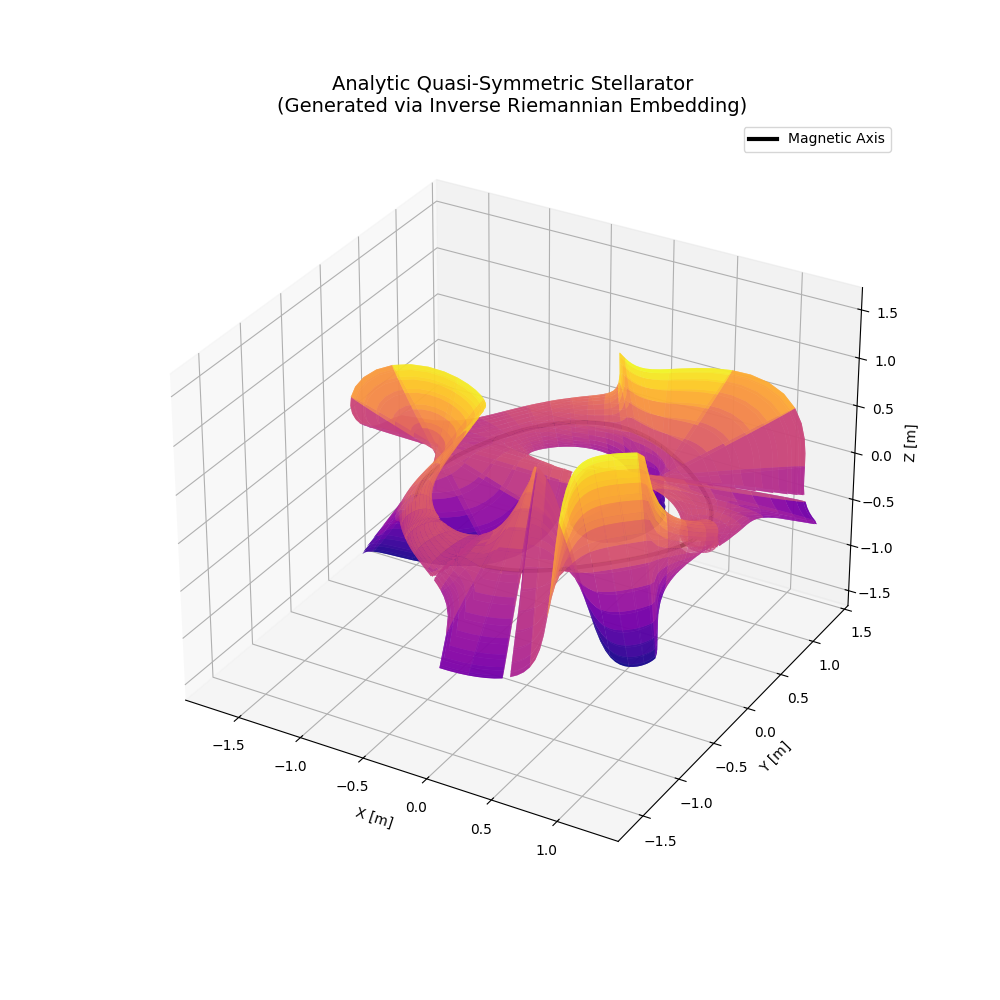
\includegraphics[width=0.8\textwidth]{stellarator_plot.png}
    \caption{Analytic Quasi-Symmetric Stellarator generated via Inverse Riemannian Embedding.}
    \label{fig:stellarator}
\end{figure}

\subsection{Geometric Validity}

The generated surface naturally exhibits rotating, elongated cross-sections in regions where axis curvature and torsion vary strongly. This is not an artifact of manual tuning but a direct consequence of the Riccati equation: the cross-section must elongate and rotate to balance curvature and torsion effects while maintaining QA consistency at the retained order.

\subsection{Engineering Implication}

Because the geometry is derived from analytic functions (smooth integration of torsion), the resulting surface is $C^\infty$ smooth. This has profound implications for the manufacturing of High-Temperature Superconducting (HTS) magnets, as it eliminates the high-frequency "ripple" often produced by discrete numerical optimization.

\subsection{Limitations of the Near-Axis Expansion}

While the NAE provides a powerful constructive method, it is formally an asymptotic expansion valid for $r \ll R_{major}$. For low-aspect-ratio configurations ($A < 4$) typical of compact reactors, second-order corrections ($O(r^2)$) become significant. Future work will extend this framework to higher orders to ensure accuracy at the plasma boundary.

Additional limitations in the present prototype include: (i) the use of $\zeta\approx\phi$ rather than tracking $d\zeta/d\phi$, (ii) the need to numerically enforce periodicity of $\sigma$ (with possible non-convergence for some axes/parameters), and (iii) the absence of a subsequent validation step against a full equilibrium solver (e.g. VMEC) and coil synthesis. These are natural next steps once candidate axes are generated.

\section{Conclusion}

This work demonstrates that intrinsic symmetry constraints can be encoded into a generating differential equation for near-axis shaping. The inverse construction yields \emph{first-order} QA-consistent cores orders of magnitude faster than traditional optimization loops for exploratory axis-family exploration and for seeding higher-fidelity workflows. Future work will extend the approach to quasi-helical symmetry, incorporate higher-order NAE terms, and validate candidate configurations against full equilibria and coil designs.

\begin{thebibliography}{9}
\bibitem{garren1991}
D. A. Garren and A. H. Boozer, ``Existence of quasihelically symmetric stellarators,'' \emph{Physics of Fluids B} \textbf{3} (1991).

\bibitem{landreman2019}
M. Landreman and W. Sengupta, ``Constructing stellarators with quasisymmetry to high order,'' \emph{Journal of Plasma Physics} \textbf{85} (2019).
\end{thebibliography}

\end{document}
